%\documentclass{brownthesis_EB}

\documentclass[final, oneside]{brownthesis_EB}

%\usepackage{Sections/CV/simplecv} %for CV section
\usepackage{Preamble}
\usepackage{hyperref}
%\usepackage{pdfpages}
\usepackage{geometry}

  
\begin{document}
    \frontmatter
    % \title{\Huge Experimental Deformation Methods' Influence on Antigorite Creep and Dehydration Behavior\\
    %  \Large Mechanical and Numerical Design of a Griggs-Type Apparatus to Better Represent the Earth.}
    \title{\Huge \textbf{Advances in Experimental Methods and Apparatus Design Applied to Investigate the Creep and Dehydration Behavior of Antigorite Serpentinite}} %Greg's title
    \author{Eric Burdette}
    \degrees{B.~S., University of Minnesota - Twin Cities, 2013}
    \dept{Earth, Environmental, and Planetary Sciences}
    \submitdate{Fall 2021}
    
    \principaladvisor{(Greg Hirth)}
    \reader{(Reid Cooper)}
    \reader{(Chris Huber)}
    \reader{(Yan Liang)}
    \reader{(Nick Beeler)}
    \dean{(Andrew G. Campbell)}
    
    % \clearpage
    % \abstract{
    % \subfile{./abstract.tex}}
    % \clearpage

    \beforepreface
    \savegeometry{main1}
    \newgeometry{lmargin=.75in,tmargin=0in}
    \prefacesection{Curriculum Vita}
        %\includepdf[pages=-]{./CV/Simple_CV_EB (1).pdf}
        \begin{figure}[h!]
            \centering
            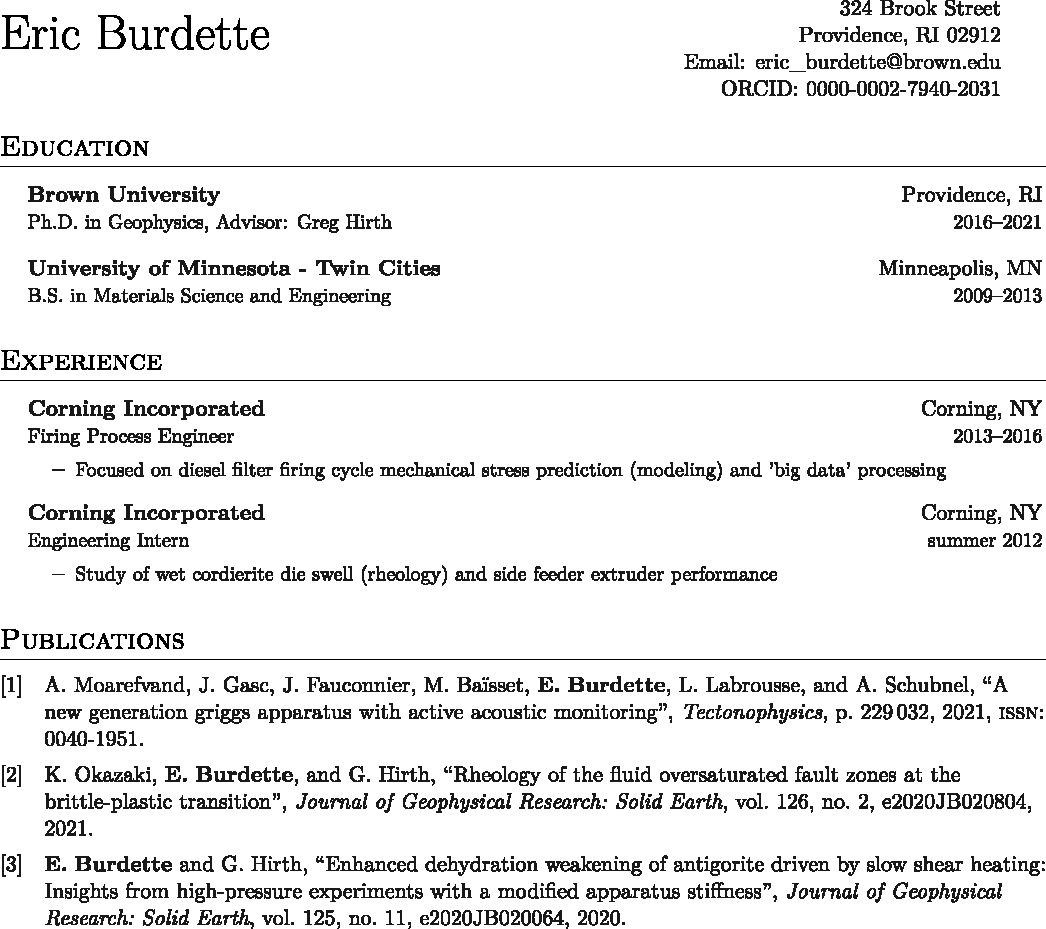
\includegraphics{Sections/CV/Simple_CV_EB (2).pdf}
            \label{fig:my_label}
        \end{figure}
    \restoregeometry{}
        
    \prefacesection{Acknowledgements}
        \subfile{Sections/Acknowledgements/Acknowledgements.tex}

    \afterpreface

    \mainmatter

    \chapter*{Introduction}
    \addcontentsline{toc}{chapter}{Introduction}
        \subfile{Sections/Introduction/Introduction.tex}


    \setlength{\parindent}{4em}

    \chapter{Enhanced Dehydration Weakening of Antigorite Driven by Slow Shear Heating: Insights from High-Pressure Experiments with a Modified Apparatus Stiffness}
        \subfile{Sections/Chapter1/ShearHeating_maintext.tex}
        %\subfile{Sections/Chapter1/ShearHeating_suppinfo.tex} %these are called in each file
    
    \chapter{Antigorite Creep at Subduction Conditions: Long Duration, High Accuracy Rheological Tests On Intact Cores Using Re-Designed Griggs Assemblies}
        \subfile{Sections/Chapter2/EB_AtgCreep_MainText.tex}
    
    \chapter{Stability of Rate-State Friction Faults in Sawcut Triaxial Geometry.}
        \subfile{Sections/Chapter3/EB_RSTriax_MainText.tex}
        
    \chapter{A Low Cost Fiber-Optic Displacement Sensor Designed For Use at High Pressure}
        \subfile{Sections/Chapter4/EB_LaserLoadCell_MainText.tex}
    

    \appendix
    \chapter{Setting up Dehydration Earthquakes in Dehydrating Antigorite: Grain Alignment (CPO) and Damage Controls Permeability and Fracture Toughness}
        \subfile{Sections/Appendix1/Atg_Align_EQs_main.tex}
        
    \chapter{Low Temperature Plastic Deformation of Confined Olivine With Free Surfaces}
        \subfile{Sections/Appendix2/EB_OlivinePillars_MainText.tex}
    
    \chapter{Griggs Assembly Thermal Structure}
        \subfile{Sections/Appendix3/EB_Thermal_Model.tex}
    
    \backmatter
    \bibliographystyle{apalike}
    \bibliography{Feb19_refs_2.bib}
    
    
\end{document}